% Implementación:
% [DONE] Falta desarrollo.
% Análisis preliminar
% [DONE] No se explica cómo se hicieron.
% [DONE] Si la idea es analizar el rendimiento de las implementaciones, para presentar la diferencia en rendimiento, es tal vez mejor mostrar sólo un gráfico de barras. En este caso, no hablan de por ejemplo, la literalidad del tiempo de ejecución o de alguna cuestión en particular en relación al crecimiento de la entrada, por lo que tal vez sería mejor cambiarlo.
% [TODO] Falta experimentación.

% [IDEA] Experimentación corta: distintas proporciones de imagen (2:1, 1:2, etc)

\section{Zoom}

El filtro LinearZoom consiste en interpolar linealmente los pixeles de la imagen, duplicando su ancho y su alto, es decir aumentando su tamaño efectivo en 4.

La interpolación lineal de los pixeles consiste en calcular los promedios de cada componente entre los pixeles adyacentes al nuevo pixel interpolado. La misma se puede representar con la siguente matriz:

\begin{table}[H]
  \centering
  \begin{tabular}{ | c | c | }
    \hline
    A & B \\ \hline
    C & D \\
    \hline
  \end{tabular}
  {\LARGE$\xrightarrow{LinearZoom}$}
  \begin{tabular}{ | c | c | c | c |}
    \hline
    A & (A+B)/2 & B & $\cdots$ \\ \hline
    (A+C)/2 & (A+B+C+D) & (B+D)/2 & $\cdots$ \\ \hline
    C & (C+D)/2 & D & $\cdots$ \\ \hline
    $\vdots$ & $\vdots$ & $\vdots$ & $\ddots$ \\
    \hline
  \end{tabular}
\end{table}

En el caso de la última fila y la última columna, como no existe información para interpolar, los elementos deben ser duplicados.

El filtro en sí no presenta un efecto visual muy notorio, pero el tamaño de la imagen crece.

\subsection{Implementación}

En la implementación en C, un detalle con el que nos cruzamos y que nos generó errores fue que la imagen se encuentra alamcenada con las filas inferiores en primer lugar. Esto es, si representamos la imagen como un arreglo bidimensonal de pixeles \texttt{RGBA** img}, esto significa que \texttt{img[0][0]} contiene el primer pixel de la fila inferior de la imagen.

Por como dividimos el problema (se detalla más adelante), esto generó confusión al implementar los casos especiales del filtro. No obstante, esto nos sirvió para estructurar mejor la implementación en ASM, que por la naturaleza de ese lenguaje resulta más compleja.

En la implementación con SIMD, podemos aprovechar las operaciones vectoriales para operar no solo sobre las múltiples componentes a la ves, sino también sobre más de un pixel (como son sumas de hasta 4 bytes, solo requerimos tamaño word por componente).

Nuestra implementación en particular procesa los pixeles en el siguiente orden (donde w es el ancho y h la altura en pixeles):

\begin{center}
  \begin{tabular}{ | c | c | c | c | c | c |}
    \hline
    w & w-1 & $\cdots$ & 3 & 2 & 1 \\ \hline
    2*w & 2*w-1 & $\cdots$ & w+3 & w+2 & w+1 \\ \hline
    $\vdots$ & $\vdots$ & $\ddots$ & $\vdots$ & $\vdots$ & $\vdots$ \\ \hline
    w*h & w*h-1 & $\cdots$ & w*(h-1)+3 & w*(h-1)+2 & w*(h-1)+1 \\
    \hline
  \end{tabular}
\end{center}

Este orden fue escogido en su momento por resultar más sencillo de implementar, pero es posible que el orden de operación resulte en menos comparaciones y saltos condicionales.

El filtro puede dividirse en 4 secciones, dependiendo de la posición en la imagen del pixel a procesar:

\begin{enumerate}
  \item Caso general: la gran mayoría de los pixeles entran en esta categoría. En estos casos, se deben cargar 4 pixeles de la memoria para procesar y crear 3 pixeles interpolados (como se muestra en la tabla anterior).

  Los 4 pixeles a procesar (que llamaremos A, B, C y D como figuran en la tabla anterior) son cargados en 2 accesos a memoria, ya que pertenecen a 2 filas distintas de la imagen de origen:

  \begin{center}
    \xmm{0} \xmmDoubleWordSmall{0}{0}{B}{A}

    \xmm{1} \xmmDoubleWordSmall{0}{0}{D}{C}
  \end{center}

  Los mismos son desempaquetados para ocupar los registros enteros en esa misma disposición.

  Por un lado, calculamos los dos pixeles que resultan de interpolar 2 pixeles de origen:

  \begin{center}

    \xmm{3} \xmmQuadWord{B}{A}

    \texttt{MOVLHPS} \xmm{3}, \xmm{3} \hfill

    \xmm{3} \xmmQuadWord{A}{A}

    \xmm{4} \xmmDoubleWordSmall{0}{0}{B}{A}

    \xmm{5} \xmmDoubleWordSmall{0}{0}{D}{C}

    \texttt{PSRLDQ} \xmm{4}, 4 \hfill

    \texttt{PSLLDQ} \xmm{5}, 4 \hfill

    \xmm{4} \xmmDoubleWordSmall{0}{0}{0}{B}

    \xmm{5} \xmmDoubleWordSmall{0}{D}{C}{0}

    \texttt{PADDB} \xmm{4}, \xmm{5} \hfill

    \xmm{4} \xmmDoubleWordSmall{0}{D}{C}{B}

    \texttt{PUNPCKLBW} \xmm{4}, CEROS \hfill

    \xmm{4} \xmmQuadWord{C}{B}

    \texttt{PADDW} \xmm{3}, \xmm{4} \hfill

    \xmm{3} \xmmQuadWord{A+C}{A+B}

    \texttt{PSRLW} \xmm{4}, 1 \hfill

    \xmm{3} \xmmQuadWord{(A+C)/2}{(A+B)/2}
  \end{center}

  Por el otro, calculamos el pixel que proviene de interpolar 4 pixeles a la vez:

  \begin{center}
    \xmm{0} \xmmQuadWord{B}{A}

    \xmm{1} \xmmQuadWord{D}{C}

    \texttt{PADDW} \xmm{1}, \xmm{0} \hfill

    \xmm{1} \xmmQuadWord{B+D}{A+C}

    \xmm{0} $\leftarrow$ \xmm{1}

    \texttt{PSRLDQ} \xmm{1}, 8 \hfill

    \xmm{1} \xmmQuadWord{0}{B+D}

    \texttt{PADDW} \xmm{1}, \xmm{0} \hfill

    \xmm{1} \xmmQuadWord{B+D}{A+B+C+D}

    \texttt{PSRLW} \xmm{1}, 2 \hfill

    \xmm{1} \xmmQuadWord{(B+D)/4}{(A+B+C+D)/4}
  \end{center}

  Por último, empaquetamos y ordenamos los pixeles de la siguiente forma:

  \begin{center}
    \xmm{2} \xmmDoubleWord{(A+B+C+D)/4}{(A+C)/2}{(A+B)/2}{A}
  \end{center}

  Al igual que en la carga, los resultados empaquetados son guardados a memoria de a 2, ya que pertenecen a distintas filas de la imagen de destino. Los dos pixeles de la parte baja del registro corresponden a la fila superior de la imagen, mientras que los dos pixeles alta del registro corresponden a la fila interior de la imagen.

  \item Última columna: en estos casos los pixeles B y D del diagrama no existen, por lo que solo se calcula 1 pixel interpolado entre A y C, y tanto A como el nuevo pixel generado son duplicados a la derecha.

  El proceso es similar al caso general, obteniendo como resultado:

  \begin{center}
    \xmm{2} \xmmDoubleWordSmall{0}{0}{(A+C)/2}{(A+C)/2}
  \end{center}

  Sin embargo, se omiten las operaciones que utilizan B y D cuando se puede, y se asumen ceros en sus lugares. Además, el pixel original se copia duplicado por separado.

  \item Última fila: similar al caso de última columna, los pixeles C y D no existen. A es interpolado con B, y tanto A como el nuevo pixel generado son duplicados hacia abajo.

  % \begin{center}

  %   \xmm{0} \xmmQuadWord{B}{A}

  %   \xmm{1} $\leftarrow$ \xmm{0}

  %   \texttt{MOVLHPS} \xmm{1}, \xmm{1} \hfill

  %   \xmm{1} \xmmQuadWord{A}{A}

  %   \texttt{PADDW} \xmm{0}, \xmm{1} \hfill

  %   \xmm{0} \xmmQuadWord{A+B}{A+A}

  %   \texttt{PSRLW} \xmm{0}, 1 \hfill

  %   \xmm{0} \xmmQuadWord{(A+B)/2}{A}

  % \end{center}

  El proceso es similar al caso general, obteniendo como resultado:

  \begin{center}
    \xmm{2} \xmmDoubleWordSmall{0}{0}{(A+B)/2}{A}
  \end{center}

  Sin embargo, se omiten las operaciones que utilizan B y D cuando se puede, y se asumen ceros en sus lugares. Ambos pixeles son duplicados en la última fila de la imagen destino.

  \item Último pixel: este caso refiere a un pixel ubicado en última fila y columna. Aqui no hay pixel para interpolar, por lo que se hace un cuadruplicado de A.

  \begin{center}

    \xmm{15} \xmmDoubleWordSmall{0}{0}{0}{A}

    \xmm{14} $\leftarrow$ \xmm{15}

    \texttt{PSLLDQ} \xmm{14}, 4 \hfill

    \xmm{14} \xmmDoubleWordSmall{0}{0}{A}{0}

    \texttt{PADDB} \xmm{15}, \xmm{14} \hfill

    \xmm{15} \xmmDoubleWordSmall{0}{0}{A}{A}

  \end{center}

\end{enumerate}

\subsection{Análisis preliminar}

Dado que la interpolación lineal es un procesamiento muy conocido de imágenes, nos esperabamos que fuese uno de los filtros más beneficiados por la vectorización de los cálculos.

\begin{center}
  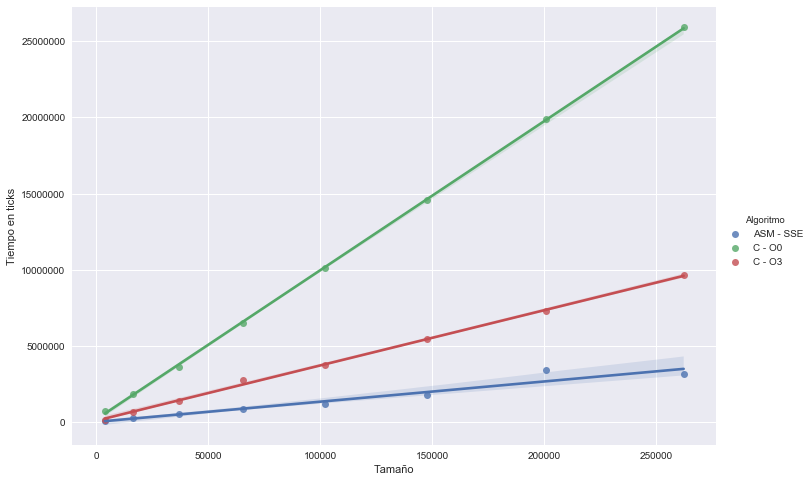
\includegraphics[scale=0.5]{img/linearZoom_CvsASMvsO3.png}
\end{center}

Por un lado, podemos observar que, como el resto de los filtros, el tiempo de ejecución de los filtros crece de forma lineal respecto a la cantidad de pixeles. Esto es esperable, ya que por cada pixel del caso general se deben leer y escribir 4 pixeles. Eso no es así para los otros pixeles, pero en nuestros tests de control estos representan la menor parte. Es posible que en imágenes pequeñas con distintas proporciones (por ejemplo, 200x50 en lugar de 100x100) esta proporción no se respete, pero el impacto de los casos borde debería ser menor a medida que crece la imagen.

\begin{center}
  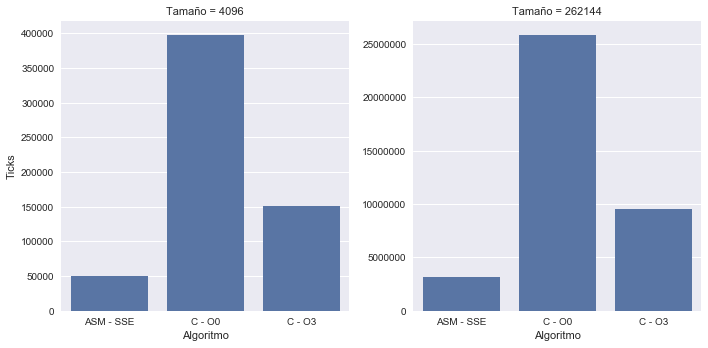
\includegraphics[scale=0.5]{img/linearZoom_CvsASMvsO3_bars.png}
\end{center}

Por otro lado, podemos ver que efectivamente, incluso con las optimizaciones de GCC, la vectorización de la interpolación aumenta el rendimiento de manera dramática, ejecutando el filtro siempre en menos del 40\% del tiempo.

\subsection{Experimentación}

TODO POR FAVOR HAGANME